%%%%%%%%%%%%%%%%%%%%%%% file template.tex %%%%%%%%%%%%%%%%%%%%%%%%%
%
% This is a general template file for the LaTeX package SVJour3
% for Springer journals.          Springer Heidelberg 2010/09/16
%
% Copy it to a new file with a new name and use it as the basis
% for your article. Delete % signs as needed.
%
% This template includes a few options for different layouts and
% content for various journals. Please consult a previous issue of
% your journal as needed.
%
%%%%%%%%%%%%%%%%%%%%%%%%%%%%%%%%%%%%%%%%%%%%%%%%%%%%%%%%%%%%%%%%%%%
%
% First comes an example EPS file -- just ignore it and
% proceed on the \documentclass line
% your LaTeX will extract the file if required
% \begin{filecontents*}{example.eps}
% %!PS-Adobe-3.0 EPSF-3.0
% %%BoundingBox: 19 19 221 221
% %%CreationDate: Mon Sep 29 1997
% %%Creator: programmed by hand (JK)
% %%EndComments
% gsave
% newpath
%   20 20 moveto
%   20 220 lineto
%   220 220 lineto
%   220 20 lineto
% closepath
% 2 setlinewidth
% gsave
%   .4 setgray fill
% grestore
% stroke
% grestore
% \end{filecontents*}
%
\RequirePackage{fix-cm}
%
%\documentclass{svjour3}                     % onecolumn (standard format)
%\documentclass[smallcondensed]{svjour3}     % onecolumn (ditto)
\documentclass[smallextended]{svjour3}       % onecolumn (second format)
%\documentclass[twocolumn]{svjour3}          % twocolumn
%
\smartqed  % flush right qed marks, e.g. at end of proof
%
\usepackage{graphicx}
\usepackage{pbox}
\usepackage{hyperref}
%
% \usepackage{mathptmx}      % use Times fonts if available on your TeX system
%
% insert here the call for the packages your document requires
%\usepackage{latexsym}
% etc.
%
% please place your own definitions here and don't use \def but
% \newcommand{}{}
%
% Insert the name of "your journal" with
\journalname{Empirical Software Engineering}
%
\begin{document}

\title{Introducing a Usage-Independent Software Quality Metric }
%\subtitle{Do you have a subtitle?\\ If so, write it here}

%\titlerunning{Short form of title}        % if too long for running head

\author{Tapajit Dey         \and
        Audris Mockus %etc.
}

%\authorrunning{Short form of author list} % if too long for running head

\institute{Tapajit Dey  \and Audris Mockus \at
            Department of Electrical Engineering and Computer Science \\  
            University of Tennessee, Knoxville \\
            Knoxville, Tennessee, USA \\
            tdey2@vols.utk.edu,  audris@utk.edu 
}

\date{Received: date / Accepted: date}
% The correct dates will be entered by the editor


\maketitle

\begin{abstract}

\keywords{First keyword \and Second keyword \and More}
% \PACS{PACS code1 \and PACS code2 \and more}
% \subclass{MSC code1 \and MSC code2 \and more}
\end{abstract}

\section{Introduction}\label{s:intro}

Software Quality has been an important factor for software developers and users alike since the beginning of software development. Today's software is a complex form of intellectual product with many different aspects, thus the term ``Quality'' has many different interpretations as well. In this paper, we look at software quality from the perspective of its users. Besides functionality and ease-of-use, an important factor for the users of a software is the number of times it crashes. A software that keeps crashing often is generally deemed to be of poor quality in terms of usability. Thus, it might sound reasonable to compare the qualities of two different softwares or two different releases of a software by comparing the total number of times it crashes. This, however, is not the right thing to do, since a software with more users is expected to see more crashes~\cite{dey2018modeling,hmps15,IQ08}. In the extreme case, a software or a release with zero users will have zero crashes, regardless of its quality. This interdependence of software usage volume and crashes experienced is often not considered in industry or in empirical studies (although few studies do note that~\cite{fenton2008using,fenton1999critique}) and may lead to misguided quality improvement efforts and/or misguided developer performance metrics. This analogy can also be extended for software defects (bugs) as well, since software crashes are manifestations of underlying defects and~\cite{caper,hmps15} observed that the number of discovered software defects increases with the number of users, although the relationship between crashes and defects is not very well understood~\cite{fenton1999critique}. 

One possible reason for this oversight is the scarcity of reliable usage data. While the number of defects and crashes reported by users are carefully tracked by most large scale projects (\textit{e.g.} Mozilla Firefox, Ubuntu etc.), tracking the variables related to usage, \textit{e.g.} the number of users, intensity of usage etc. is almost impossible to track without a reliable monitoring system. Such a system is rarely used by open-source softwares and even many traditional software-as-a-product systems do not or can not have such capability. Moreover, even when such a dataset is available, it is almost always proprietary, so obtaining and sharing it, even for the software development teams in these proprietary projects, is difficult since the deployment is typically managed by a different team within the organization. Without such data, however, it becomes exceedingly difficult to interpret the quality of a software from the customer reported crashes/defects alone due to the interdependence of usage and crashes/defects~\cite{dey2018modeling,hmps15,IQ08}.

We were able to obtain the usage data for several mobile applications developed by Avaya, \textit{viz.}  Avaya Communicator for Android and iOS (currently known as Avaya Equinox\textregistered) and Avaya one-X\textregistered  Mobile SIP iOS Client. The usage data was obtained from Google Analytics. By analyzing the usage data for these applications we establish the interdependence between the number of crashes and usage, and propose a quality metric that is independent of usage, which would enable us to compare the qualities of different softwares and/or different releases of a software more accurately. 

We used three usage related variables: number of users, 
usage intensity (average duration of software use per user), and usage frequency 
(average number of times the app was used by a user), along with two variables describing attributes 
of the particular release: release date and effective duration of the release, measured by how 
long the release continued to have new users, and looked at how these variables affect 
the number of exceptions \textit{i.e.} application crashes.  

After the usual data cleaning and variable construction stages, we first applied a linear regression (LR) model to identify the significant predictors for the number of exceptions. Then we used a Bayesian Network (BN) model to discover the interrelationship between the variables. The BN model was generated by using structure search algorithms, and the search method was chosen based on the result of a simulation study. We have presented the detailed result of the simulation study and hope that other practitioners willing to use BN structure search methods in their work might find it useful.  Finally, we ran a random forest (RF) model to identify the importance of the variables for predicting the number of exceptions. All analyses in this study was done in R~\cite{R}. We found that the frequency and intensity of usage have little impact on the number of exceptions, but the number of users does have a significant impact. 

In our previous work~\cite{dey2018modeling}, we only analyzed the General Availability releases for  Avaya Communicator for Android. Since the data was collected through similar means, we had the same set of variables. We found similar results from that study as well, with the number of new users being the most important factor affecting the number of exceptions.
In that study, we proposed a quality metric of average number of exceptions experienced by end users (so lower means better) and found it to be independent of other usage metrics. However, directly using the number of exceptions per user fails to differentiate between two softwares/releases which have zero exceptions but different number of users. Although the observed quality is same for these two, the one with more users is expected to be more robust, and thus should be considered to be of better quality. To address this problem, we propose that instead of directly using the number of exceptions per user, we should instead take a Bayesian approach and calculate the probability of an user encountering an exception. The metric could be initialized with a non-informative or weakly informative prior, or the quality metric value from the last release could be used as a prior. This adds a little bit of complexity in calculation, but finally gives us a more complete and reliable quality metric. We present both the simpler quality metric and our new, a slightly more complex metric in this paper, because, in some cases the complexity adds more overhead to the calculation than it adds value to the measurement. We discuss the merits and demerits of both, and leave the choice of the metric to the judgment of the analysts who are better aware of the  demands of a particular situation.

We have also applied our method of analysis to a very different scenario of NPM packages. Node Package Manager (NPM) is the package manager for node.js, an open-source, cross-platform JavaScript run-time environment. 
Since we do not have the number of crashes for these packages, we looked at the number of issues reported for these packages instead.
NPM tracks the number of downloads of the packages, and while the number of downloads counted by NPM is essentially a mix of downloads by users, bots, and mirror servers, as explained in~\cite{npmdl}, it is the closest measure of usage we could find for open-source projects. We only looked at the NPM packages that have more than 10,000 downloads a month. While according to ~\cite{npmdl}, automated downloads are expected to be around 50 per day, or 1500 per month, we wanted the usage to be high enough to have a noticeable impact on the number of issues reported, so we set the threshold to 10,000. 

Result NPM

In summary, we have established the relationship between the number of exceptions (crashes) and usage by analyzing different softwares, and have proposed a Bayesian quality metric that gives a more complete and reliable measure of quality. We have also used our approach to study the relationship between the number of downloads and issues of NPM packages. (found) 
Finally, we have presented the detailed result of the simulation study we conducted to choose the best performing BN structure search algorithms, which we believe will of of use to practitioners willing to use BN structure search methods in their work.

The rest of the paper is organized as follows: In Section~\ref{s:relwork}, we discuss the related works and other studies that have found similar results. In Section~\ref{s:soft}, we give some details about both the commercial software and NPM packages we analyzed. Details of the data collected for the study is discussed in Section~\ref{s:data}. Section~\ref{s:datapre} lists the data preprocessing steps we followed. We discuss the simulation study we performed for choosing the best performing BN structure search method that was used in subsequent analysis in Section~\ref{s:sim}. In Section~\ref{s:explain}, we present the different modeling approaches used to explain the number of exceptions(crashes) and the results. The simpler quality metric we used is discussed in Section~\ref{s:qual} and the new, more complex metric is discussed in Section~\ref{s:qualnew} along with the related analysis results. We discuss the merits and demerits of the two metrics in Section~\ref{s:comparequal}. The result of the analysis of the NPM packages is presented in Section~\ref{s:npm}. We discuss the implications of our result in Section~\ref{s:implication}. Finally, we discuss the limitations of our study in Section~\ref{s:limitation} and conclude the paper in Section~\ref{s:conclusion}.  

\section{Related Work}\label{s:relwork}



\section{Software Studied}\label{s:soft}

For this study, we looked into two different types of software, which are vastly different in nature. The primary focus of the study is on the commercial software developed by Avaya for mobile applications, which are from the telecommunication domain. For external validation of the theory developed using this data, we looked into the NPM packages, which are mostly open-source JavaScript packages used in web-development. In this section, we provide some details about the two to help contextualize our study.

\subsection{The Mobile Applications developed by Avaya}
One of the software chosen for this study was Avaya Communicator for
Android and iOS (currently known as Avaya Equinox\textregistered ). It
integrates the mobile devices of the users with their office Avaya
Aura\textregistered communications environment and delivers mobile
voice and video VoIP calling, cellular call integration, rich
conferencing, instant messaging, presence, visual voicemail,
corporate directory access and enterprise call logs\footnote{\url{https://support.avaya.com/products/P1574/avaya-equinox-for-android}\\   \url{https://support.avaya.com/products/P1597/avaya-equinox-for-ios/All}}.

Another software we studies was the Avaya one-X\textregistered Mobile  SIP  for  iOS, which provides mobile communications for the iPhone, iPod touch, and iPad through a wireless-enabled SIP Avaya Aura\textregistered environment combining enterprise features with the convenience of a mobile endpoint for users on the go. The Avaya one-X Mobile\textregistered SIP for iOS appears as an end point in the Aura\textregistered environment\footnote{\url{https://support.avaya.com/products/P0949/avaya-onex-mobile-sip-for-ios}}.

Avaya is developing large, complex, real-time software systems that
are embedded and standalone products. Development and testing are
spread through 10 to 13 time zones in the North America, USA, Europe
and Asia. R\&D department employed many virtual collaboration tools
such as JIRA, Git, WIKIs and Crucible. Development teams use
Scrum-like development methodologies with a typical 4-week
sprint. We consider a 15+ year old software component, the so-called
Spark engine.  As a software platform, Spark provides a consistent
set of signaling platform functionalities to a variety of Avaya
telephone product applications, including those of third parties.
Spark is a client platform that provides signaling manager, session
manager, media manager, audio manager, and video manager. The
codebase involves more than 200K files and, over all forks, over 4M
commits.  The Android software chosen for this study is a fork of
the Spark codebase. A more in-depth description of the development
process is provided in~\cite{amhp14}.

\subsection{NPM Packages}



\section{Details of the Data}\label{s:data}

\subsection{Data on mobile applications collected from Google Analytics}
The post-deployment data for this application was obtained from the 
Google Analytics platform.
Google Analytics is a web analytics service offered by
Google that tracks and reports website traffic. It is now one of the most
widely used web analytics services on the internet. In addition to
traditional web applications it also allows tracking of mobile
applications. To do that, the producer of a mobile application needs
to set up an account and instrument their mobile application to send certain
events to Google Analytics. Notably, it works for the mobile
applications investigated in this study. 

We collected data for a number of mobile applications developed by Avaya from Google Analytics, but some of the datasets turned out to be unusable for this study, for reasons ranging from very low volume of collected data (\textit{e.g.} Avaya Communicator for Android - Experimental Releases) to zero recorded exceptions making an analysis impractical (\textit{e.g.} Avaya One-X\textregistered   ScsCommander ). The following datasets were found usable:
\begin{itemize}
    \item Avaya Communicator for Android - General Availability and Development versions.
    \item Avaya one-X\textregistered Mobile  SIP  for  iOS - General Availability versions.
    \item Avaya Communicator for iOS - General Availability versions : This only had 6 releases, so it wasn't used for the modeling, we applied our calculated Quality metrics on it for testing. 
\end{itemize}

The data was collected between December 2013 and May 2016, although the exact time varies across the applications. Although we are primarily focused on the General Availability (GA) versions, since only these versions are available for end-users, we also decided to look into the development version for Avaya Communicator for Android, since we have detailed data available for these versions and we wanted to see if it shows a different characteristics from the GA versions.  

The original data obtained from Google Analytics had measures for the variables 
listed in Table~\ref{t:measures}, aggregated at a per-day granularity, meaning 
that each entry in the original data table contained the measures for the numerical 
variables (marked with a $\dagger$ symbol in the table) for each unique combination
of date, application release version, operating system version, mobile device brand, 
category, and model. We had the same set of variable for all the applications listed above.

It is important to note that Google Analytics releases only
aggregate data even to developers of the application and limits the
number of REST API calls, so one can not, for example, retrieve
usage data for every calendar second or get exact time of the
events. The daily counts split by release version of
the application, OS version, and type of device, provided
sufficiently fine granularity for our analysis. 
\begin{table}
\caption{Measures available in the Original Data}\label{t:measures}
\begin{tabular}{|p{6.5cm}|p{4cm}|}\hline
Application Release Version & No. of exceptions$\dagger$\\\hline
Operating System version in the user's device &Date of record entry\\\hline
No. of fatal exceptions$\dagger$& No. of new visits$\dagger$\\\hline
No. of visits$\dagger$ & Time on site$\dagger$\\\hline
\pbox{6cm}{Details on user's mobile device:\\ brand, category(mobile or tablet) and model} & No. of new users$\dagger$\\\hline
No. of total users$\dagger$& Sessions per user$\dagger$\\ \hline
\end{tabular}
\vspace{-10pt}
\end{table}

\subsection{Data on NPM Packages}


\section{Data Preprocessing}\label{s:datapre}

This section contains the data cleaning, transformation, and variable 
construction steps undertaken prior to the application of the different modeling 
methods. 

\subsection{The Google Analytics data for the Mobile Applications}

\textbf{Removal of variables before aggregation: } Upon initial
investigation into the data, we found that no. of exceptions and
no. of fatal exceptions were exactly the same, as recorded by Google
Analytics, so we removed the no. of fatal exceptions from the
dataset. Only fatal exceptions were recorded for this application,
i.e., crashes that require a complete restart of the mobile
application and, potentially, may affect the operating system
itself.  This is not surprising since the bulk of the functionality
for the application was written in C$++$ and called from the mobile OS
via Native Interface.

We did not consider the variables related to mobile device
details and operating system versions because the
application, as noted above, was primarily written in C$++$ and the
user interface aspects that vary greatest among devices and versions
of OS were not likely to have influence. To validate that
assumption we investigated and found no
correlation of exceptions with either variable. 

\noindent
\textbf{Data correction:}
This additional prepossessing step was not a part of our previous study~\cite{dey2018modeling}.
We found during careful inspection of the data that some of the releases had non-zero number
of users but zero new users in the dataset. This obviously hints at some part of the data 
being missing. So, as a data correction step, we modified the number of new users so that 
in the chronological order of the data, the cumulative number of new users is never 
less than the number of users for a day.

\noindent
\textbf{Aggregating data to per-release granularity:}
We had some missing values in the data, however, most of the missing data was about the
mobile devices and since we didn't use them in our analysis, we got rid of that
problem by simply dropping the variables. Since our aim is to model the quality of the
different releases, we aggregated the data to a per-release 
granularity, from the the original data that was recorded in per-day granularity. 
The raw data contained 177 different GA releases. We dropped 4 of
them from further consideration because a significant
portion of observations were missing. The result of aggregation, however,
was two new variables: start date (first day for which we have a
record for that release) of a release, and end date (last date for
which we have a record for that release) of a release, which in turn
helped create another variable: duration of a release. We did
not to keep the end date in the final table, since duration and
start date can be used to compute the end date.

\noindent
\textbf{Verifying the correctness of Release date:}
The original data involves only the usage aspects and the version
information of the software. The project under consideration was
relatively new and it was one of the early attempts for the team to deploy
mobile software on Android and iOS. As such, not everything
was well documented and also was rapidly evolving over time  and no
record of the exact release dates for most of the releases was
available. We did manage to get release dates for some of releases
from Google Play Store/ Apple App Store, but not all the release dates  were
available.  For the releases with dates available on Google Play
Store/ Apple App Store, the official release dates from Avaya records, and the start
dates obtained from the data were either very close or exactly the
same, so we do not have a reason to doubt the dates obtained from the
data. 

\noindent
\textbf{Removal  of variables post aggregation:}
The numerical variables were aggregated to give a sum for each
variable. Upon further inspection, we found the number of users, new
users, visits, and new visits to be highly correlated. In the second
iteration, we removed the variable ``sessions per user'', because
aggregating it directly is meaningless, and we were not sure how it
was originally calculated by Google Analytics (was it a mean or
a median? were new users or total users counted?). We also removed
the ``total users'' and ``total visits'', because while summing up the
new users/visits for each day gives an accurate measurement of the total
number of new users/visits for a release, it is not guaranteed that
summing up total users/visits does the same due to possible double
counting the number of users/visits. 

\noindent
\textbf{Final list of variables:}
Keeping the goal of our study in mind, the variables we have after the initial cleaning 
steps give us necessary information for a model of post-release defects and software usage.
In our list of variables, we have the total number of exceptions \textit{i.e.} post-release defects. 
As for measures related to software usage, we have the total number of new users;
the ``Time.On.Site'' variable, normalized by the number of users of a release,
provides a measure for the temporal intensity of usage per user;
and the number of visits per user is a measure for the frequency of usage.
We also have two variables related to each individual release: the start date \textit{i.e.} the release
date gives a measure for the calender time of each release, and is useful in gaining insight
about if the number of post-release defects and software usage vary with time, and 
the duration of a release, which could have an effect on the number of exceptions
and the number of new users, since these variables were not normalized with duration.
Since we only have a limited amount of data, we restricted ourselves to use only 
these six variables.
Our final aggregated data table had the measures listed in Table~\ref{t:finalvarss}, 
with the corresponding variable names we used in the model enclosed in brackets. 

\begin{table}
\caption{Measures in the Aggregated Data Table}\label{t:finalvarss}
\begin{tabular}{|l|l|}\hline
\pbox{6cm}{\textit{Release variable} - Start Date \\for the release (Release.Date)} & \pbox{6cm}{\textit{Release variable} - Effective Duration \\of the release (Release.Duration)}\\\hline
\pbox{6cm}{\textit{Post-Release defects} - \\Total No. of exceptions (Exceptions)}  &  \pbox{6cm}{\textit{Usage variable} - Average\\ time on site per user (Usage.Intensity)}\\\hline
\pbox{6cm}{\textit{Usage variable} -Total\\ number of new users (New.Users)} & \pbox{6cm}{\textit{Usage variable} \\- No. of visits per user (Usage.Frequency)}\\\hline
\end{tabular}
\vspace{-15pt}
\end{table}

\noindent
\textbf{Log-transformation of variables:}
The release date was converted from the Date format to numeric format, which 
resulted in the values for the release date variable being represented by the 
difference in days from Unix time (counted from 1970-01-01).
We found that all of the variables under consideration
had a long-tailed distribution, so we took logarithm of them. Final distribution of the variables in available in our GitHub repository:\\ \url{https://github.com/tapjdey/release\_qual\_model}.


\section{Simulation Study for Selecting the Best BN Structure Search Method}\label{s:sim}

\subsection{Basics of Bayesian Network models}
Bayesian Network~\cite{koller2009probabilistic,scutari2010introduction} 
is a type of Probabilistic Graphical Model (PGM), which explicitly represents the
conditional dependency/independence as a directed acyclic graph where variables
represent nodes and dependencies represent links, and thus this
representation can be used as a generative model\footnote{A
  generative model specifies a joint probability distribution over
  all observed variables, whereas a discriminative model
  (like the ones obtained from regression or decision trees) provides a
  model only for the target variable(s) conditional on the predictor
  variables. Thus, while a discriminative model allows only sampling
  of the target variables conditional on the predictors, a
  generative model can be used, for example, to simulate
  (i.e. generate) values of any variable in the model, and
  consequently, to gain an understanding of the underlying mechanics
  of a system, generative models are essential.}.  
Bayesian Networks models can be useful in the context of Software Engineering research~\cite{fenton1999critique} due to having several advantages over
regression models. To be precise, regression analysis is a very
simple BN where there is one directed link from each independent variable
to dependent variable. BNs, therefore, can help with 
multicollinearity, a common problem with software engineering 
data~\cite{yu2002predicting,subramanyam2003empirical,briand2000exploring,Changes07}, 
that is present in our data as well, by linking independent variables. 

Another variety of PGM that we did not use in this paper 
(details in Section~\ref{s:limitation}) is the Markov random
fields that represent the interrelationships between variables 
as undirected graphs. They differ in the set of
independencies they can encode and the factorization of the
distribution that they induce~\cite{koller2009probabilistic}.

\noindent\\
\textbf{Bayesian Network Model construction:}
Despite the promises of BNs, they tend to be quite sensitive to data,
and operational data, is often problematic~\cite{M14,zmz15}. 
Careful preprocessing, therefore, is needed to ensure a 
reliable and reproducible result. Two primary ways to use BNs exist. With the first
approach the graph represents dependencies obtained from domain experts.
The graph may include prior distributions
about the parameters of the overall model. The data is then used to
calculate the posterior distribution and to make inference. The
second approach puts minimal a-priori assumptions about the model
and focuses on the search for the best graphical representation for a given dataset
(structure learning). This is an NP-hard problem~\cite{chickering1996learning},
but a number of different heuristic structure learning algorithms are
available. Due to the lack of any strong theory connecting the variables we are considering,
we decided to use the structure search method for BN model construction.
Since our goal is to find a Bayesian network model for the data, we didn't
examine the methods that do not result in a Directed Acyclic Graph
(DAG). We found that the \textit{bnlearn} package in R implements a wide range of BN searching
methods for continuous, discrete, or a mixed set of variables and
the corresponding families of scoring functions and also has a good number of examples.
These methods were also shown to be able to recover the underlying network for a 
protein-signaling-chain (in Biology) in~\cite{bnppt}. We, therefore,
use this package for our analysis. In addition to the methods
implemented in \textit{bnlearn} package, we investigated some 
methods from a few other packages which can be interfaced with
the \textit{bnlearn} package.

Due to the potential inconsistencies of the BN models, we performed our 
modeling in two stages. First, we considered all available BN structure 
methods in the \textit{bnlearn} package and ran a simulation based study to 
find the methods that are most accurate and then we used those methods on our 
data to create the final model.

\noindent\\
\textbf{Methods considered:}\\
The different BN structure search methods we considered are listed below:

\begin{itemize}
\item \textit{Greedy search algorithms}(HC)~\cite{nagarajan2013bayesian,bnppt}
\item \textit{Hybrid algorithms}(Hybrid)~\cite{nagarajan2013bayesian,bnppt}
\item \textit{Posterior maximization} using \textit{deal} package in R~\cite{bnppt,dealR} .
\item \textit{Simulated Annealing} using \textit{catnet} package in R~\cite{catnetR,bnppt}.
\item \textit{MAP (maximum a posteriori estimation) Bayesian Model Averaging} (MAP) ~\cite{nagarajan2013bayesian,bnppt}
\end{itemize}

All structure search algorithms try to maximize some form of a network score. 
Among the various scores available, BIC score is the suitable one when 
the goal is to create an explanatory model from non-informative prior models
~\cite{shmueli2010explain,sober2002instrumentalism}.
BIC score is used for discrete data while the Gaussian 
equivalent of BIC (bic-g) score is used for continuous data.

The results, structure and parameters resulting from a structure
search algorithm are often noisy, meaning that
different settings induce slightly different networks. To mitigate
this effect we use non-parametric bootstrap model averaging method
described in~\cite{friedman1999data}, which provides confidence
level for both the existence of edge and its direction. This enables
us to select a model based a confidence threshold. Authors
of~\cite{friedman1999data} argue that threshold is domain specific
and needs to be determined for each domain. For instance, a threshold of 
 0.95 indicates that  only the edges that appeared in more than
 95\% of the bootstrap optimized models were selected. 
 
Many applications of BNs discretize the data prior to applying
the structure learning methods, so we considered it as a possibility as well.
Using continuous data works best
when the random variables (possibly after a transformation) 
have Gaussian distribution. While using
discrete data does not require such assumptions, obtaining the optimal
discretization for a dataset is in itself an NP-hard
problem~\cite{chlebus1998finding}. Choosing a
sub-optimal discretization technique may result in spurious or
missed relationships, which can in turn result in incorrect
dependencies being reported in the resulting model. Given the pros
and cons of both types of methods, we use methods of both types for
our simulation study. As we are interested in creating a generative model, we had to
use a discretization method that is unsupervised. The basic problem
with commonly used supervised methods (\textit{e.g.} Chi-square, or
MDLP discretization algorithms) is that they optimize
discretization to improve explanatory power for 
a single response variable. This is not suitable for a 
PGM structure search, because we do
not know  which variables will be responses (have arrows
pointing to them) and which will be independent (have no incoming
arrows) {\em a-priori}. While some research on multidimensional
discretization methods exists~\cite{perez2006supervised},
we are not aware of any that have a robust implementation.

\noindent\\
\textbf{Simulation Study:}\\
\begin{figure}
\centering
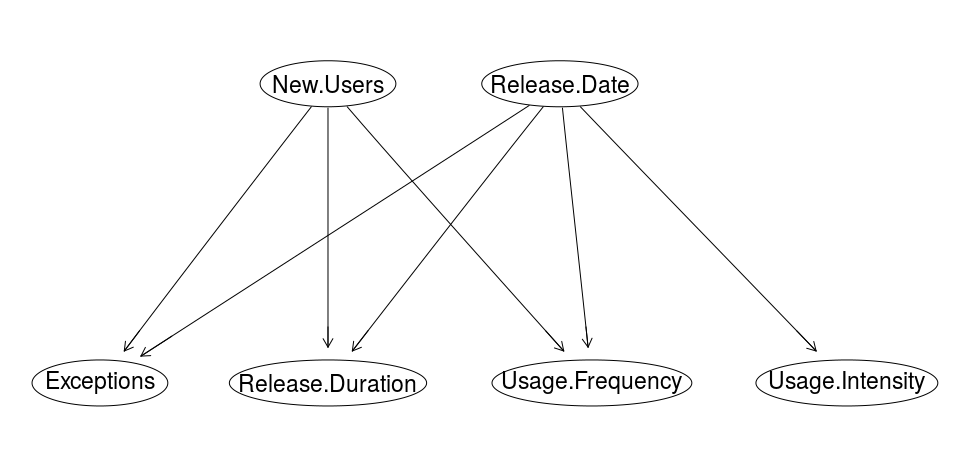
\includegraphics[width=\linewidth]{custom}
\caption{Custom model used for Simulation Study}
\label{fig:theory}
\end{figure}
We performed the simulation study by first creating 
a random BN (see Figure~\ref{fig:theory}) with 
six nodes, since we also have six variables in our final list (Table~\ref{t:finalvarss}).
For demonstration purposes we use the same variable names. 
We fitted this graph with our data (log-transformed and scaled) to generate values for the coefficients 
for each edge. This model was used in our simulation study going forward.
We created 1000 different datasets from the BN structure in Figure~\ref{fig:theory},
and applied the different structure search algorithms 
(both continuous and discrete versions, where available) listed above. Our performance metric
is finding how many times can the different algorithms recover the 
underlying structure from the simulated data. 

Other than testing the methods themselves, we also tested whether or not we should 
discretize the data. We tried different discretization methods, \textit{viz.} 
equal interval, equal frequency, and
k-means clustering based discretization methods from the
\textit{arules} package~\cite{arulesR}, and the 
Hartemink\footnote{Hartemink's pairwise mutual information 
method\cite{hartemink2001principled}.} discretization methods 
in the \textit{bnlearn} package.

Except for the \textit{Posterior maximization} using \textit{deal} package, 
all other results were bootstrapped, so we tested different thresholds in our 
simulation study as well. Finally, for the the Hybrid search algorithm, in which
conditional independence tests are performed to restrict
the search space for a subsequent greedy search, there are many restrict methods
available, \textit{viz.} gs" (Grow-Shrink), "iamb" (IAMB), "fast.iamb" (Fast-IAMB), "inter.iamb" (Inter-IAMB), "mmpc" (Max-Min Parent Children), "si.hiton.pc" (Semi- Interleaved HITON-PC), "chow.liu" (Chow-Liu), "aracne" (ARACNE)~\cite{bnlearnR}, and we tested all of these restrict options 
in our simulation study. 

\begin{table}
\caption{Result of Simulation Study}\label{t:sim_result}
\begin{tabular}{lll}
\hline
\textbf{Method} & \textbf{Exact} & \textbf{Off-by-one} \\ \hline
HC & 0.574 & 0.264 \\
MAP & 0.596 & 0.214 \\
Hybrid- si.hiton.pc & 0.000 & 0.019 \\
Hybrid- mmpc & 0.000 & 0.016 \\
Hybrid- gs & 0.000 & 0.011 \\
HC-D-F & 0.000 & 0.010 \\
Hybrid- iamb & 0.000 & 0.010 \\
Hybrid- mmpc -D-H & 0.000 & 0.008 \\
Hybrid- si.hiton.pc -D-H & 0.000 & 0.008 \\
HC-D-H & 0.000 & 0.007 \\
Hybrid- mmpc -D-F & 0.000 & 0.007 \\
Hybrid- si.hiton.pc -D-F & 0.000 & 0.006 \\
Hybrid- iamb -D-F & 0.000 & 0.005 \\
Hybrid- gs -D-F & 0.000 & 0.004 \\
Hybrid- gs -D-H & 0.000 & 0.004 \\
Hybrid- iamb -D-H & 0.000 & 0.002\\\hline
\end{tabular}
\end{table}

The result of the simulation study is shown in Table~\ref{t:sim_result}, which shows 
the fraction of times exact structures and off-by-one structures\footnote{one extra 
/ missing / reversed edge} were generated by each method in the simulation. The result varies 
with the chosen threshold, but in Table~\ref{t:sim_result}, we show the overall performance of
different methods and we only show 
the methods which generated an exact or off-by-one structure at least once in the simulation.
For the hybrid search methods, we list mention the restrict option that was used, and the 
`-D' suffix indicates a discretization method was used to discretize the data prior to applying 
a structure search method. `-D-H' indicates Hartemink discretization method and `-D-F' indicates 
Equal-Frequency discretization method. It is clear from the table that only HC and MAP methods
can effectively reproduce the correct underlying structure around half of the times and they create 
more off-by-one structures than others, indicating the error rate is the lowest for these methods.

\begin{table}
\caption{Result of Simulation Study: Different Thresholds}\label{t:sim_threshold}
\begin{tabular}{llll}
\hline
Method & Threshold & Exact & Off-by-one \\ \hline
MAP & 0.85 & 0.68 & 0.25 \\
MAP & 0.80 & 0.67 & 0.25 \\
MAP & 0.90 & 0.67 & 0.26 \\
MAP & 0.95 & 0.66 & 0.27 \\
MAP & 1.00 & 0.66 & 0.27 \\
MAP & 0.75 & 0.66 & 0.21 \\
HC & 0.65 & 0.63 & 0.23 \\
HC & 0.70 & 0.63 & 0.23 \\
HC & 0.75 & 0.63 & 0.23 \\
HC & 0.80 & 0.63 & 0.23 \\
HC & 0.85 & 0.62 & 0.24 \\
HC & 0.55 & 0.62 & 0.23 \\
HC & 0.60 & 0.62 & 0.23 \\
MAP & 0.70 & 0.62 & 0.21 \\
HC & 0.90 & 0.60 & 0.26 \\
MAP & 0.65 & 0.58 & 0.17 \\
HC & 0.95 & 0.57 & 0.29 \\
MAP & 0.60 & 0.43 & 0.14 \\
MAP & 0.55 & 0.33 & 0.11 \\
HC & 1.00 & 0.19 & 0.47\\ \hline
\end{tabular}
\end{table}

In Table~\ref{t:sim_threshold}, we show the fraction of times exact and 
off-by-one models were generated by HC and MAP methods for different thresholds. 
It can be seen that using a moderately high threshold between 0.75 and 0.9 gives
good results for both HC and MAP, while higher thresholds for HC and lower thresholds for MAP
give worse results. Using the optimal threshold creates models that have more than one wrong 
and/or missing edge only 7-14\% of the times. 

The result of the simulation study had the following findings:
\begin{itemize}
\item Using structure search algorithms on the continuous data resulted in much more frequent recovery of the original BN structure compared to discretized data.
\item Bootstrapping  improves the stability of the results considerably.
\item The bootstrapped Hill-Climbing search and MAP Bayesian Model Averaging algorithms outperformed all others both in terms of accuracy and runtime, being able to recover the underlying structure more than 63\% of the times and making no more than one error 86\% of times with optimal thresholds. 
\end{itemize}

We consider this study one of the contributions of the paper, and hope that it 
would be useful for researchers using BN structure learning techniques.

\section{Explaining Exceptions for the Commercial Software}\label{s:explain}
As mentioned earlier, we conducted our analysis in three stages: first, we used linear regression (LR) on the data with the number of exceptions as the response variable; then, we used Bayesian Network (BN) modeling approach to identify the interrelationship between the variables; and finally, we used a random forest (RF) model to verify the results. 

We chose LR for the simplicity, robustness and ease of interpretation. To better understand interrelationships among variable (since LR is not applicable for sets of highly correlated predictors) we used BN models. Finally, to establish the 
predictive capabilities of our models we used RF, which is known as one of the best Machine Learning classifiers. That way we could both obtain the most insight and also to validate our findings through the use of radically different approaches.


\section{Application of our model: A derived measure of Quality}\label{s:qual}


\section{The New Quality Metric}\label{s:qualnew}


\section{Comparison of the Two Quality Metrics}\label{s:comparequal}


\section{Analysis of the NPM Data: Results}\label{s:npm}


\section{Implication of our Findings}\label{s:implication}


\section{Limitations}\label{s:limitation}



\section{Conclusion}\label{s:conclusion}


%\begin{acknowledgements}
%If you'd like to thank anyone, place your comments here
%and remove the percent signs.
%\end{acknowledgements}

% BibTeX users please use one of
%\bibliographystyle{spbasic}      % basic style, author-year citations
\bibliographystyle{spmpsci}      % mathematics and physical sciences
%\bibliographystyle{spphys}       % APS-like style for physics
\bibliography{reference.bib}   % name your BibTeX data base

\end{document}
% end of file template.tex

